\documentclass[tikz]{standalone}
\begin{document}
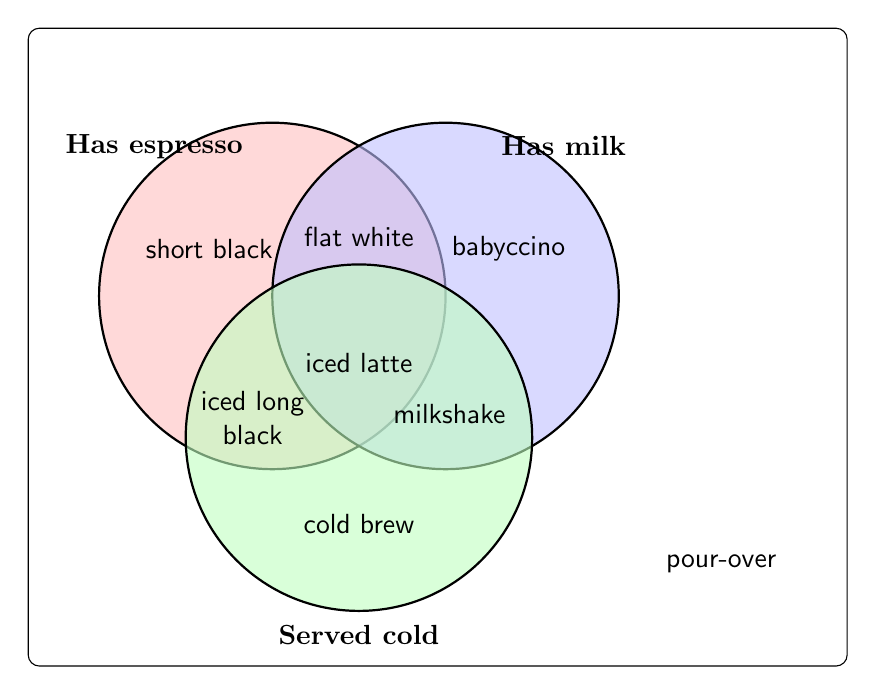
\begin{tikzpicture}[font=\sffamily]
  % bounding box / outside region
  \draw[rounded corners] (-4.2,-4.1) rectangle (6.2,4.0);

  % circles
  \draw[thick,fill=red!25,fill opacity=0.6]    (-1.1,0.6) circle (2.2);
  \draw[thick,fill=blue!25,fill opacity=0.6]   ( 1.1,0.6) circle (2.2);
  \draw[thick,fill=green!25,fill opacity=0.6]  ( 0.0,-1.2) circle (2.2);

  % labels
  \node[font=\bfseries] at (-2.6,2.5) {Has espresso};
  \node[font=\bfseries] at ( 2.6,2.5) {Has milk};
  \node[font=\bfseries] at ( 0.0,-3.7) {Served cold};

  % drinks
  \node at (-1.9, 1.2) {short black};       % espresso only
  \node at ( 1.9, 1.2) {babyccino};         % milk only
  \node at ( 0.0,-2.3) {cold brew};         % cold only
  \node at ( 0.0, 1.35) {flat white};       % espresso + milk
  \node[align=center] at (-1.35,-0.95) {iced long\\black};  % espresso + cold
  \node at ( 1.15,-0.9) {milkshake};        % milk + cold
  \node at ( 0.0,-0.25) {iced latte};       % all three
  \node at ( 4.6,-2.8) {pour-over};         % outside all
\end{tikzpicture}
\end{document}
